\documentclass[a4paper,french]{paper}
\usepackage{../../_latex_assets/villemejane_iogs_ceti}

%Informations about this document 
%------------------------------------------
\def\module{Ingénierie Electronique pour le Traitement de l'Information}
\def\moduleAbrege{6N-047-SCI / IéTI}
\def\annee{}

\def\titre{TD 1 / Diodes et sources à LEDs}
\author{Julien VILLEMEJANE}

\subtitle{TD 1}
\institution{LEnsE / Institut d'Optique Graduate School}

\title{\titre}
\begin{document} 
%Beginning First Page. 
%------------------------------------------
\enteteThematiqueObligatoire{}

%Beginning Content. 
%------------------------------------------
\vspace{-1cm}
%%%%%%%%%%%%%%%%%%%
\encadreTDExo{1 - Caractéristique d'une diode}{
On rappelle le symbole et le sens des courants et tensions aux bornes d'une diode :

\begin{center}
	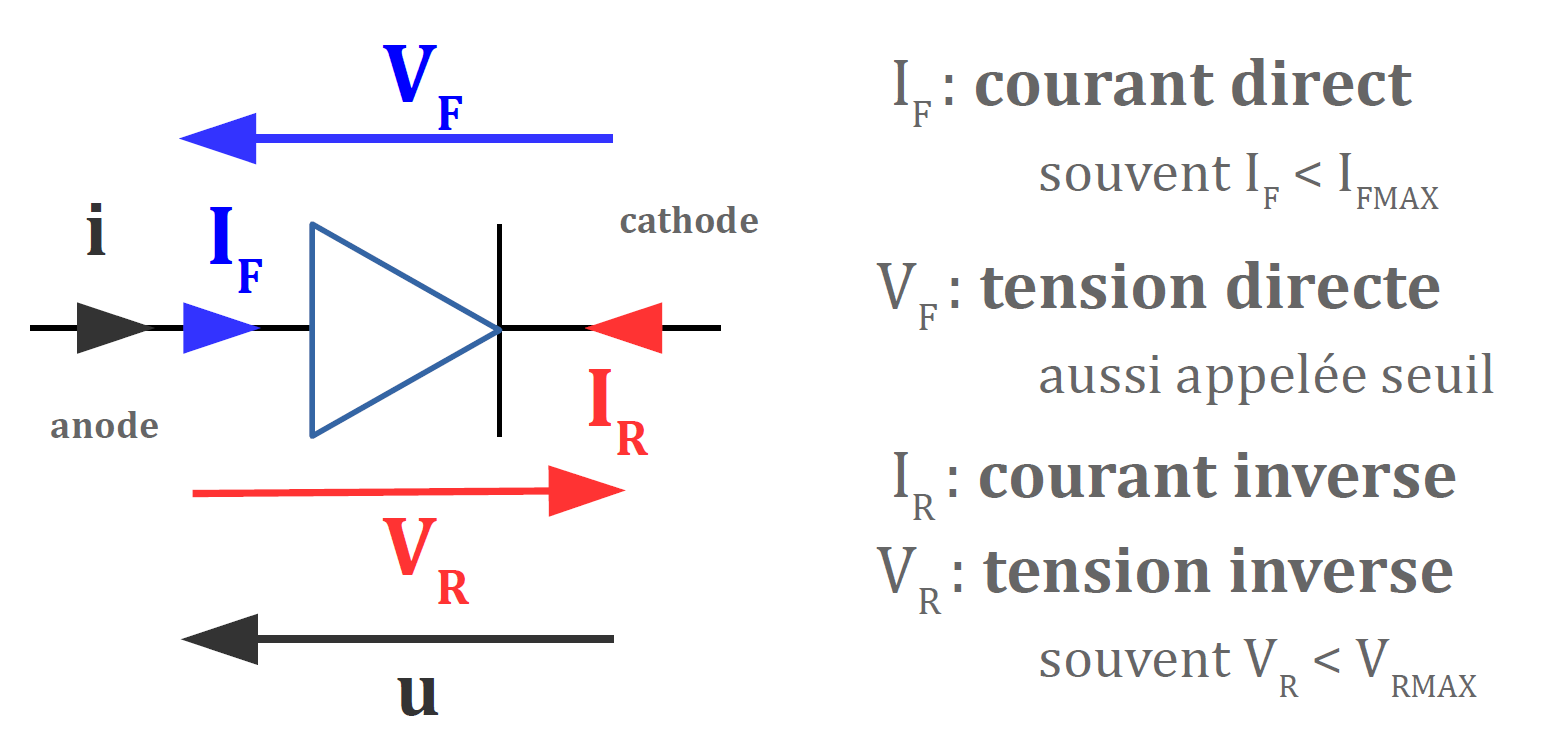
\includegraphics[width=8cm]{images/diodes_000.png}
\end{center}

\medskip
On fournit la documentation technique d'une LED Rouge "classique" (\textit{Kingbright L-53HD}).

\begin{enumerate}
	
	\item Trouvez et relevez la \textbf{caractéristique $I(V)$} de cette LED (allure).
	\item Relevez et commentez l'ensemble des \textbf{paramètres électriques}.
	\item De quel(s) paramètre(s) dépend l'\textbf{intensité lumineuse} émise ?

\end{enumerate}
}

\textbf{\large Caractéristique statique}

Dans la documentation technique, on trouve la figure suivante : 

\begin{center}
	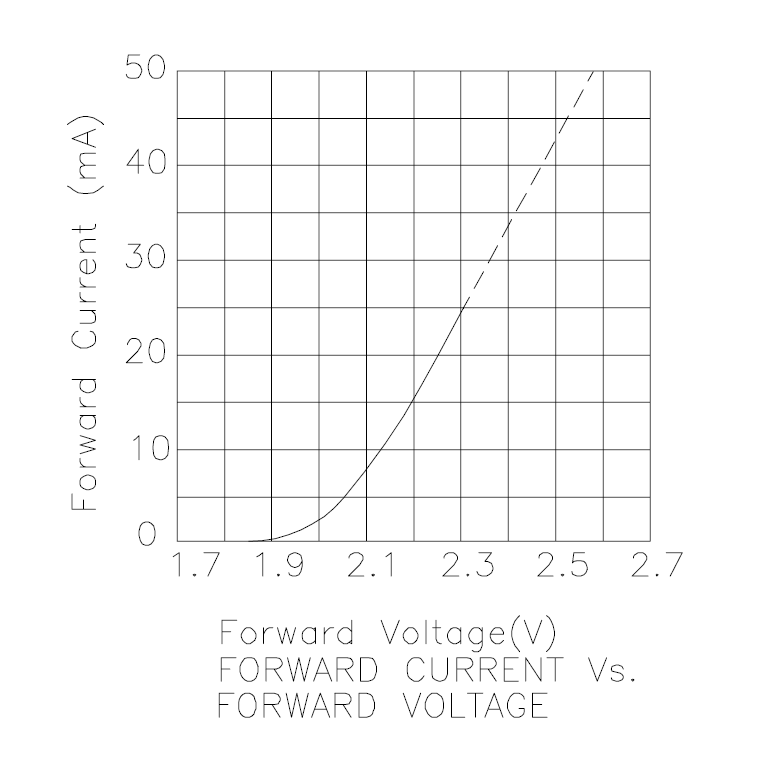
\includegraphics[width=10cm]{images/TD/caract_001_b_cor.png}
\end{center}


\textbf{\large Caractéristiques électriques et optiques}

On peut s'intéresser à la figure suivante : 

\begin{center}
	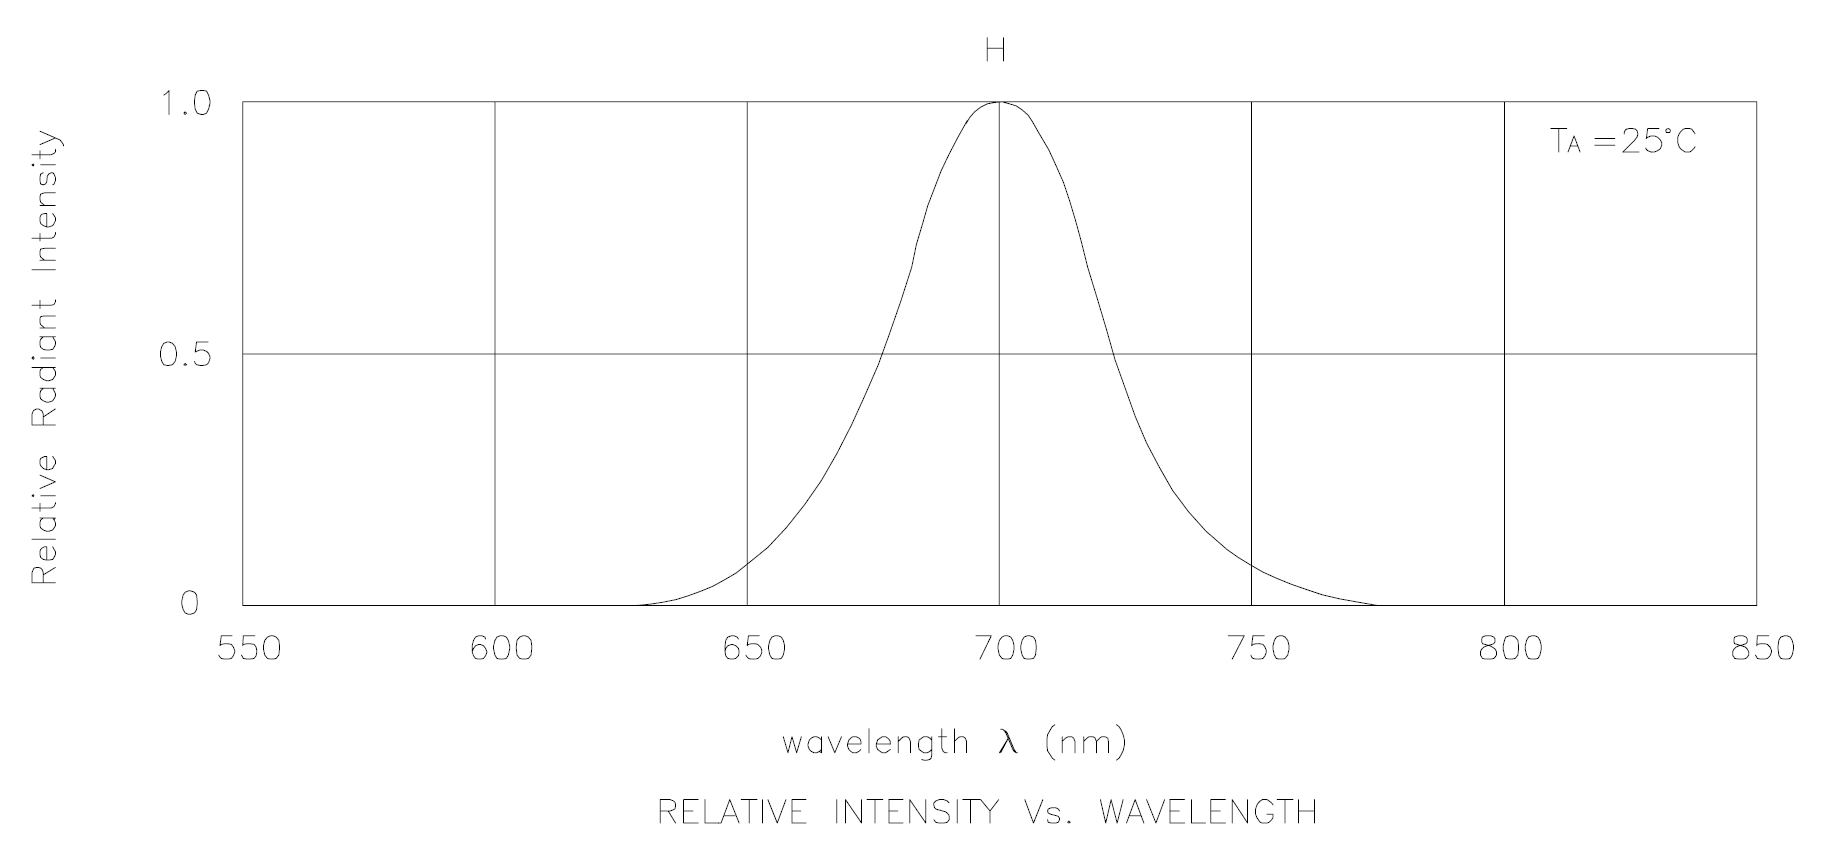
\includegraphics[width=8cm]{images/TD/caract_001_c_cor.png}
\end{center}

\begin{itemize}
	\item \textbf{$\lambda{}_{peak}$} : longueur d'onde de la LED - ici $\lambda{}_{peak} = 700\operatorname{nm}$
	\item $\Delta\lambda{}_{1/2}$ : "bande-passante" lumineuse de la LED, telle que l'intensité soit supérieure à la moitié de l'intensité maximale - ici $\Delta\lambda{}_{1/2} = 45\operatorname{nm}$ (donnée pour des conditions expérimentales spécifiques - $I_F = 20\operatorname{mA}$ courant nominal)
	\item capacité "parasite" / C : capacité à ajouter en parallèle au modèle de la LED (jonction PN)
	\item \textbf{tension directe} $V_F$ : il s'agit de la différence de potentiel directe apparaissant aux bornes de la LED lorsque le courant nominal est atteint - ici $V_F = 2.25\operatorname{V}$ pour $I_F = 20\operatorname{mA}$
	\item courant inverse $I_R$ : courant apparaissant dans la LED lorsqu'elle est soumise à une tension inverse $V_R = 5\operatorname{V}$
	
	\item \textbf{puissance dissipable} : puissance que va pouvoir dissiper la LED - ici $P = 120\operatorname{mW}$
	\item \textbf{courant direct admissible} $I_F$ : courant direct que peut laisser passer la diode sans destruction - ici $I_{FMAX} = 25\operatorname{mA}$
	\item courant direct impulsionnel $I_{Fpeak}$ : courant direct temporaire que peut laisser passer la diode sans destruction - ici $I_{FMAXpeak} = 130\operatorname{mA}$ - sous certaines conditions : durée maximale d'application de $0.1\operatorname{ms}$ avec un rapport cyclique de 1/10 (soit un temps de repos de $0.9\operatorname{ms}$)
	\item tension inverse admissible $V_R$ : différence de potentiel maximale que peut supporter la LED en inverse
\end{itemize}



\textbf{\large Emission de photons}

	D'après la documentation technique, on peut voir que l'intensité lumineuse dépend :
	\begin{itemize}
		\item du courant direct - lien proportionnel
		\item de la température ambiante
	\end{itemize}
	
	\begin{center}
		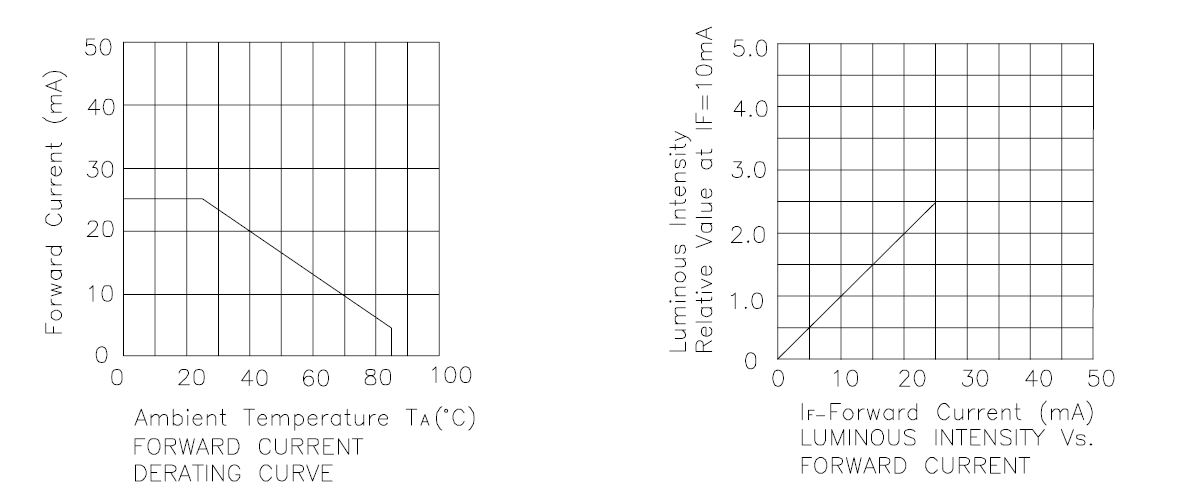
\includegraphics[width=12cm]{images/TD/caract_001_d_cor.png}
	\end{center}


\newpage
%------------------------------------------
%%%%%%%%%%%%%%%%%%%
\encadreTDExo{2 - Redressement à diodes}{

Soient les circuits suivants :

\begin{center}
	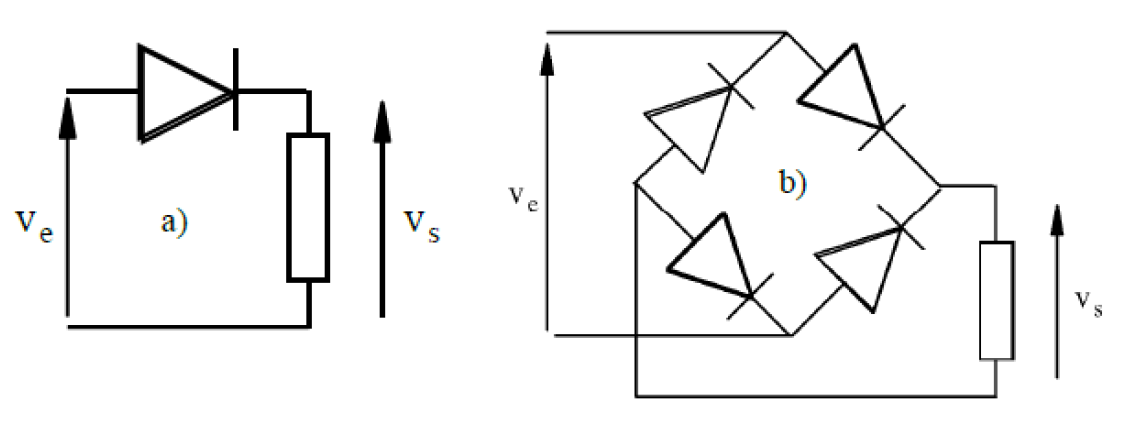
\includegraphics[width=8cm]{images/TD/redresseur_001_a.png}
\end{center}

Donnez l'allure du signal de sortie $V_S(t)$ des circuits a et b suivants pour un signal d'entrée de forme sinusoïdale telle que $V_e(t) = A \cdot sin(\omega{}t)$ dans le cas d'une diode idéale. Puis dans le cas d'une diode avec une tension de seuil $V_d$. On supposera que $A > V_d$.

}


\begin{center}
		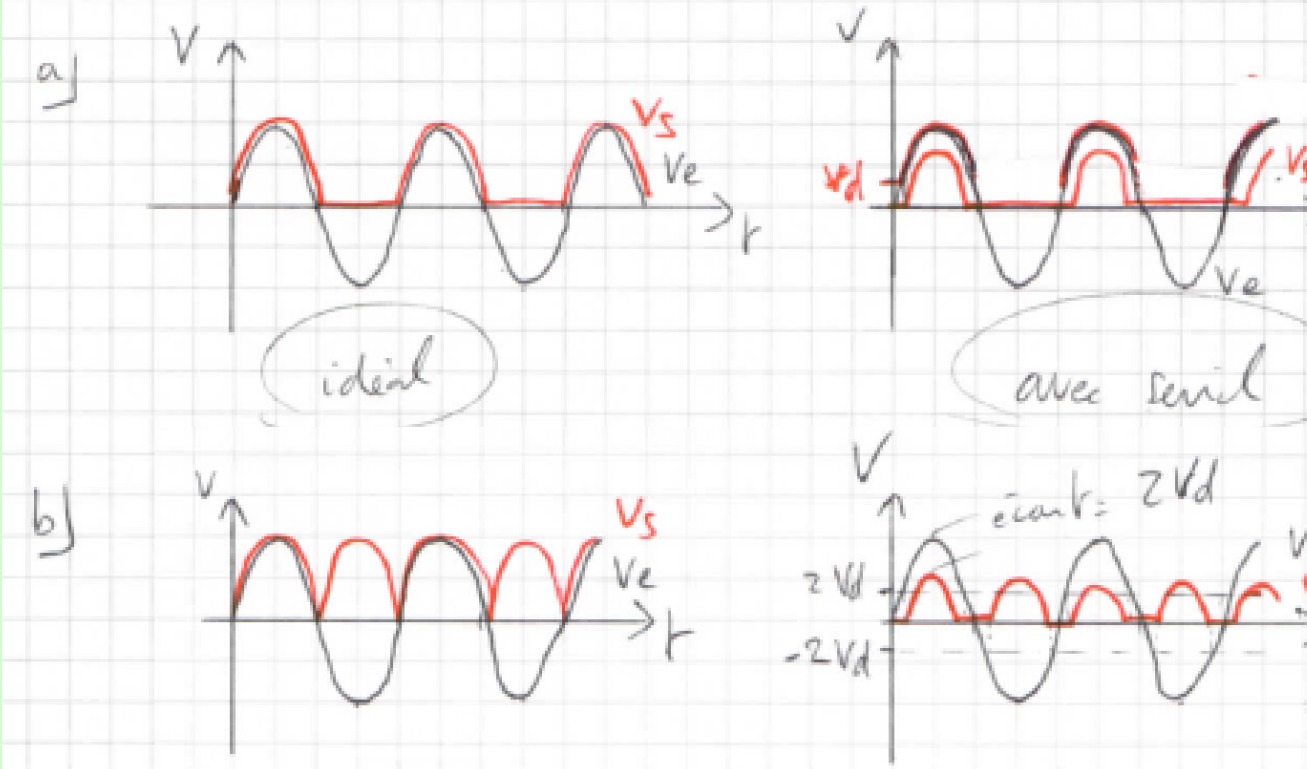
\includegraphics[width=8cm]{images/TD/redresseur_001_a_cor.png}
	\end{center}
	
	On peut également simuler ce montage à l'aide du logiciel LTSpice (par exemple - fichier de simulation disponible sur eCampus et sur le site du LEnsE). On obtient alors, dans le cas d'une diode "classique", la figure suivante - cas (a) à gauche et cas (b) à droite ($A = 10\operatorname{V}$ et $f = 10\operatorname{Hz}$ - en haut les tensions $V_E(t)$ et $V_S(t)$ et en bas le courant dans la diode pour le cas (a) et dans la résistance R pour le cas (b)) :

	\begin{center}
		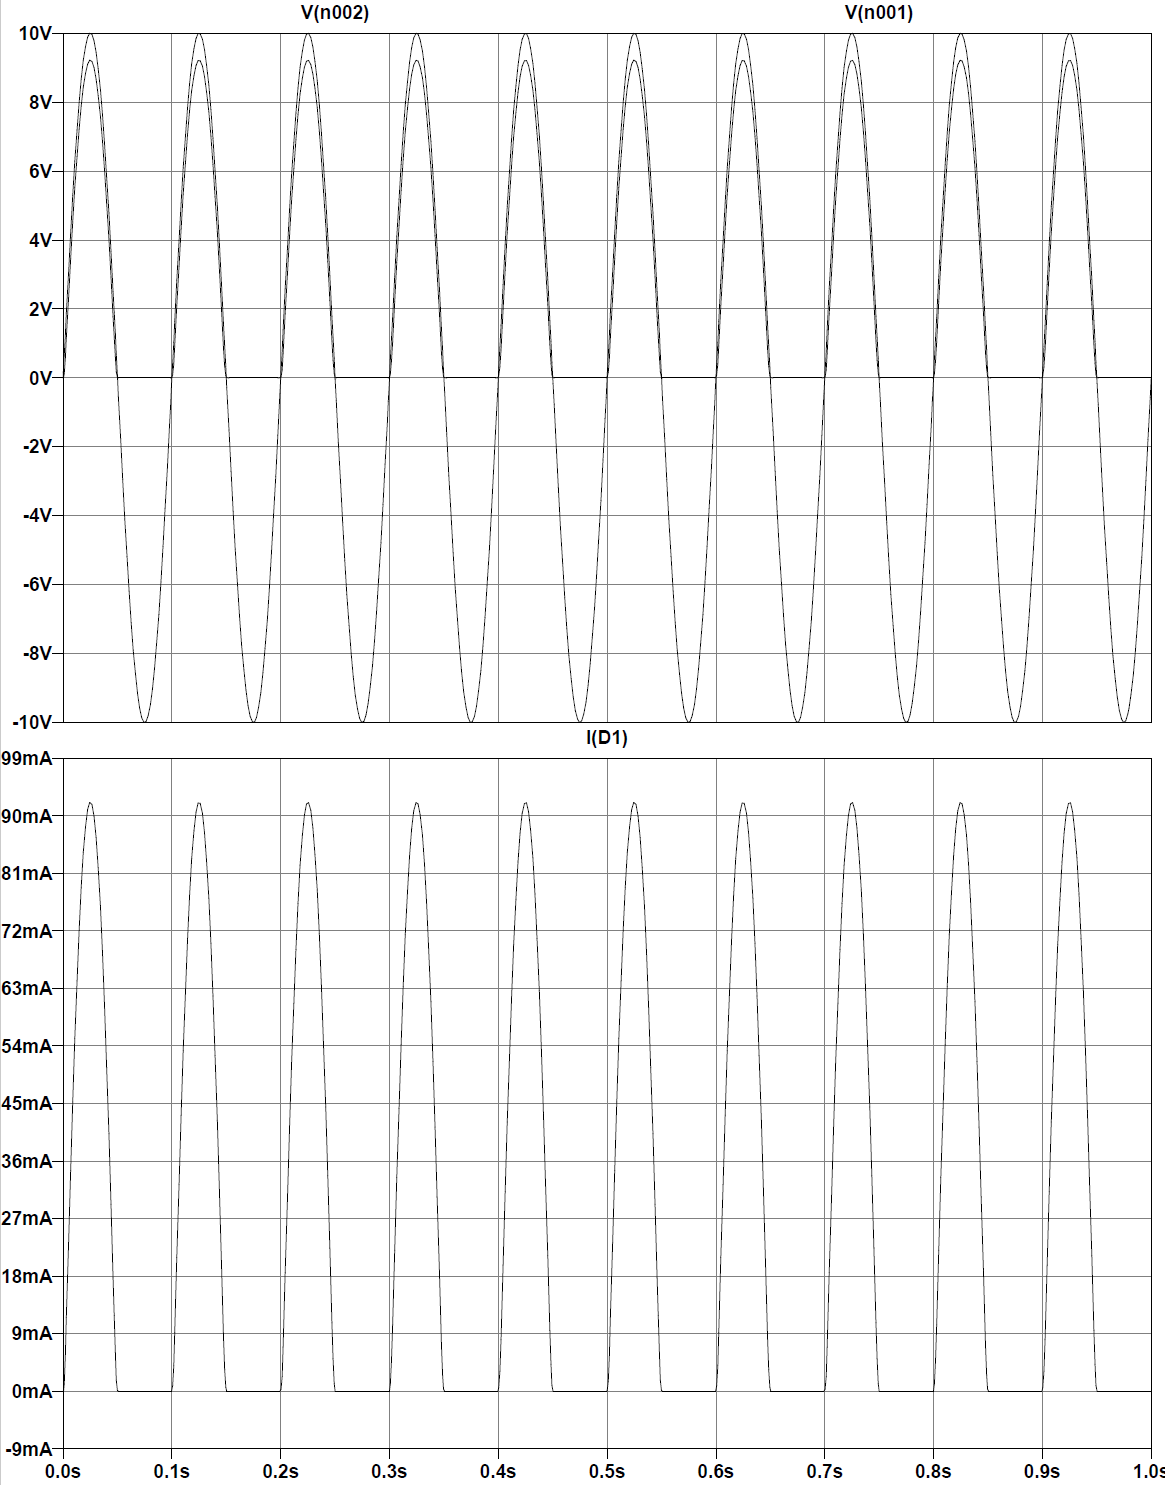
\includegraphics[width=6cm]{images/TD/redresseur_001_b_cor.png}\hfill
		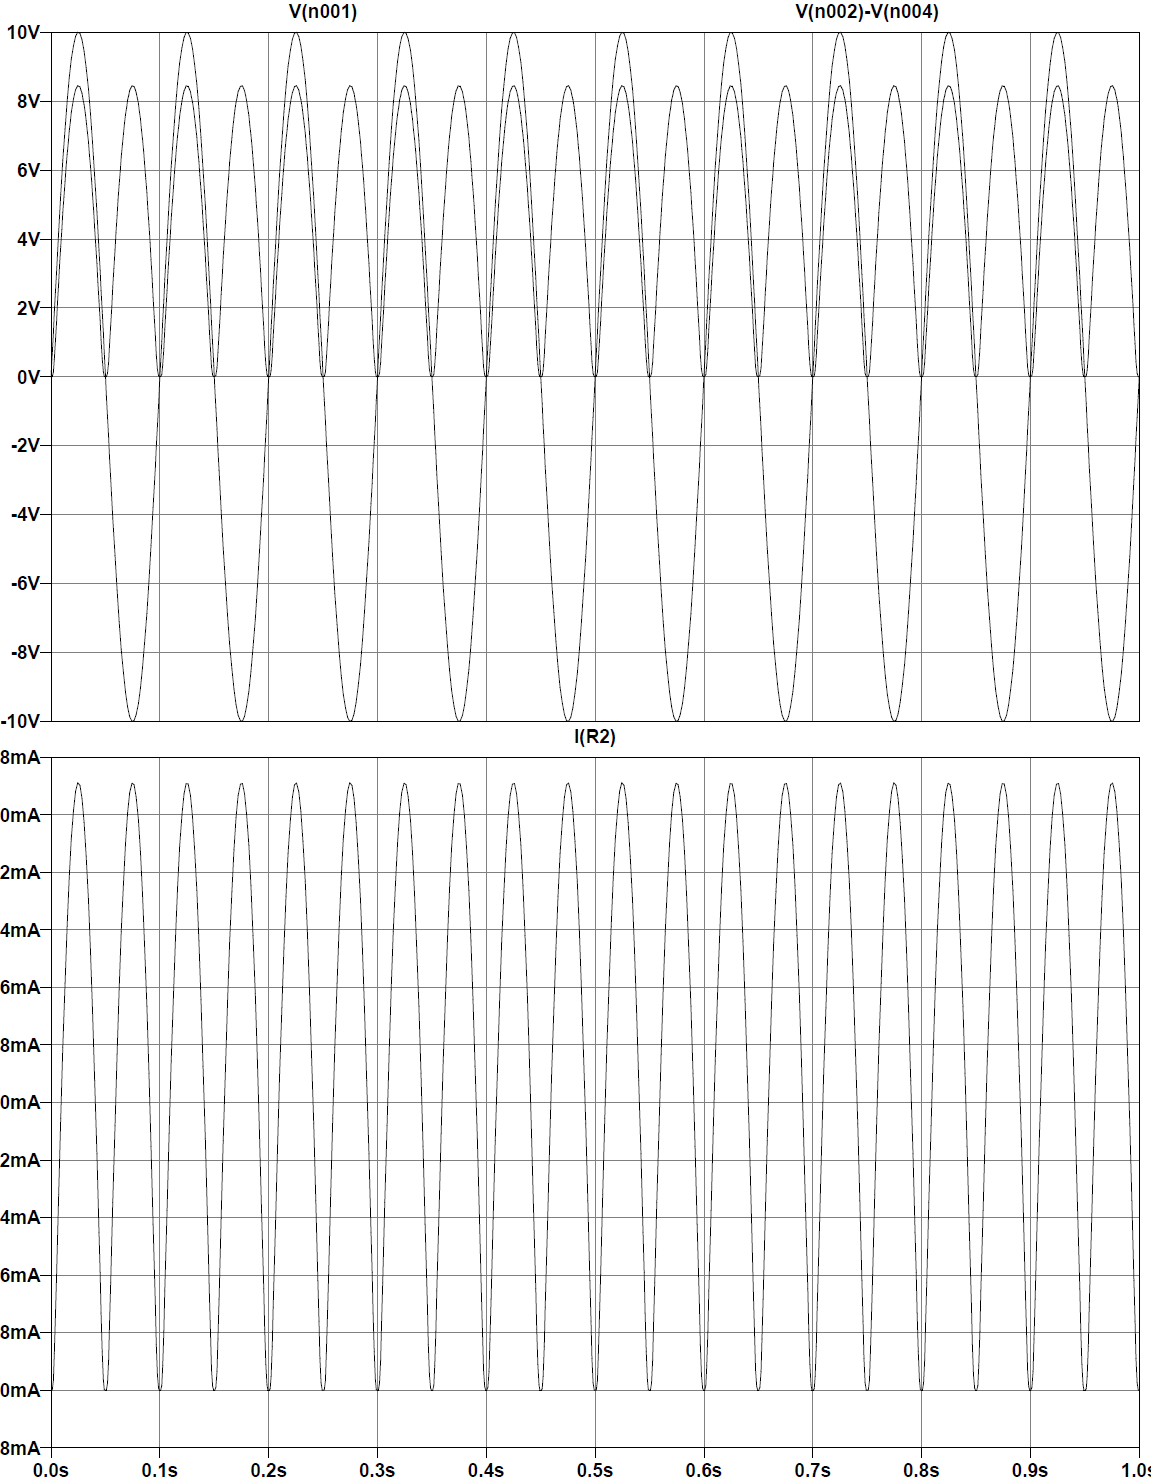
\includegraphics[width=6cm]{images/TD/redresseur_001_c_cor.png}
	\end{center}	
	
	
	
\newpage
%------------------------------------------
%%%%%%%%%%%%%%%%%%%
\encadreTDExo{3 - Générateurs de signaux}{

On considère à présent les deux montages suivants :

\begin{center}
	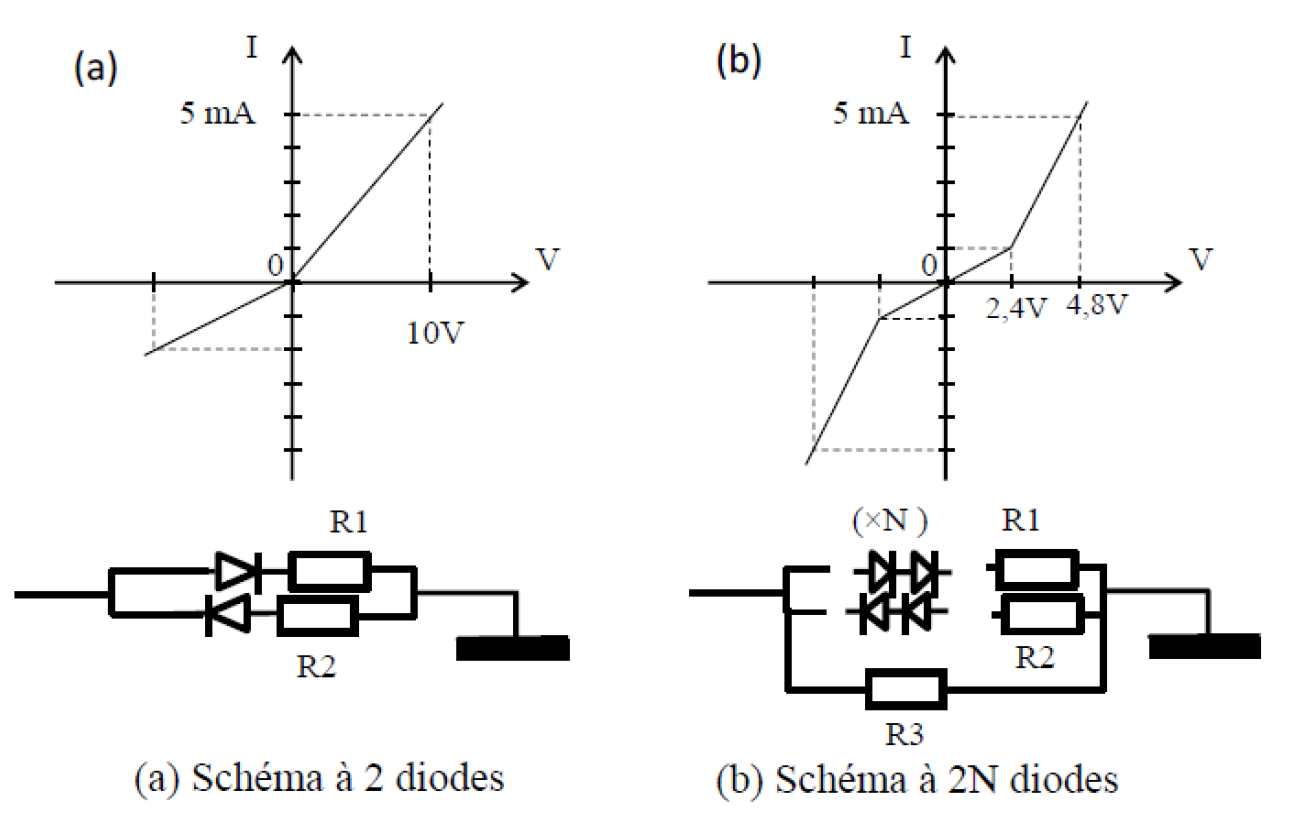
\includegraphics[width=12cm]{images/TD/diodes_002_a.png}
\end{center}

\begin{enumerate}
	\item Dans le cas du montage de la figure (a) et d'utilisation de diodes parfaites et idéales, que doivent valoir $R_1$ et $R_2$ pour obtenir la caractéristique tracée dans le graphe $I(V)$ ?
	\item Dans le cas du montage de la figure (b), les diodes ont pour seuil $0,6\operatorname{V}$. Que doivent valoir $R_1$, $R_2$ et $R_3$ et le nombre de diodes $N$ ($N = 2$ a été dessiné arbitrairement) pour obtenir la caractéristique tracée dans le graphe $I(V)$ ?
\end{enumerate}
}

\textbf{\large 1 - Montage figure (a)}

$R_1$ donne la pente lorsque $V < 0$, on a alors : $R_1 = \Delta{}V=\Delta{}I = 10/5 \cdot 10^{-3} = 2\operatorname{k\Omega}$

De même, $R_2$ donne la pente lorsque $V > 0$, on a alors : $R_2 = \Delta{}V=\Delta{}I = 10/2 \cdot 10^{-3} = 5\operatorname{k\Omega}$



\textbf{\large 2 - Montage figure (b)}

Entre $-2.4\operatorname{V}$ et $+2.4\operatorname{V}$, seule la résistance $R_3$ intervient, les diodes des autres branches sont bloquées. On a alors : $R3 = \Delta{}V=\Delta{}I = 2.4 / 10^{-3} = 2.4\operatorname{k\Omega}$

\medskip

Pour un changement de comportement à $+2.4\operatorname{V}$, il faut au total $N = 4$ diodes en série ($4 \cdot 0.6\operatorname{V} = 2.4\operatorname{V}$).

\medskip

Les pentes avant $-2.4\operatorname{V}$ et après $2.4\operatorname{V}$ étant les mêmes, $R_1 = R_2$

De plus, dans cette zone-là, $R_1 // R_3 = R_1 \cdot R_3 / (R_1 + R_3) = \Delta{}V=\Delta{}I = 2.4 / 4 \cdot 10^{-3} = 600\operatorname{\Omega}$

Ainsi, $R_1 = 800\operatorname{\Omega}$.

%------------------------------------------
%%%%%%%%%%%%%%%%%%%
\encadreTDExo{4 - Emetteur à LED}{
On souhaite réaliser un montage émetteur à l'aide de la diode rouge de l'exercice 1. On propose d'étudier le montage suivant :

\begin{center}
	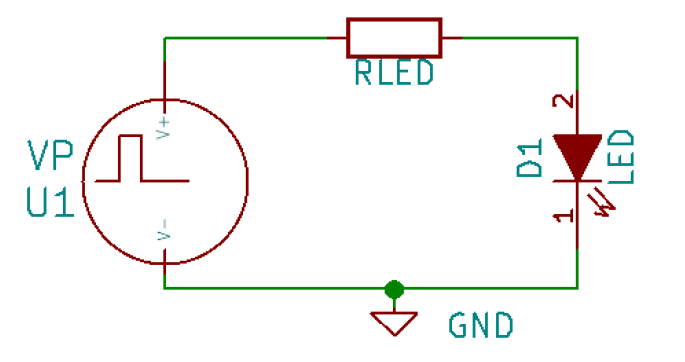
\includegraphics[width=8cm]{images/TD/emetteur_003_a.png}
\end{center}

\begin{enumerate}
	\item Cas 1 : La source de tension $V_P$ est une source continue. Elle délivre une différence de potentiel de $5\operatorname{V}$.
	\begin{enumerate}
		\item Quelle est la valeur maximale du courant que la diode peut supporter dans ces conditions ?
		\item Quelle est la valeur minimale que doit avoir $R_{LED}$ pour respecter cette condition ?
		\item Quel sera alors le courant moyen qui traversera la LED ?
	\end{enumerate}
	
	\item Cas 2 : La source de tension $V_P$ est une source impulsionnelle. Elle délivre des impulsions de $5\operatorname{V}$ de durée $0.1\operatorname{ms}$ avec une fréquence de répétition de $1\operatorname{kHz}$.
	\begin{enumerate}
		\item Quelle est la valeur maximale du courant que la diode peut supporter dans ces conditions ?
		\item Quelle est la valeur minimale que doit avoir $R_{LED}$ pour respecter cette condition ?
		\item Quel sera alors le courant moyen qui traversera la LED ?
	\end{enumerate}

	\bigskip
	
	On s'intéresse maintenant à une LED infrarouge (IR) de type SFH415 (documentation fournie en annexe). 

	\item Cas 2bis : La source de tension $V_P$ est une source impulsionnelle. Elle délivre des impulsions de $5\operatorname{V}$ de durée $0.1\operatorname{ms}$ avec une fréquence de répétition de $1\operatorname{kHz}$.
	\begin{enumerate}
		\item Quelle est la valeur maximale du courant que la diode peut supporter dans ces conditions ?
		\item Quelle est la valeur minimale que doit avoir $R_{LED}$ pour respecter cette condition ?
		\item Quel sera alors le courant moyen qui traversera la LED ?
		\item Quelle sera la puissance dissipée dans la résistance $R_{LED}$ ?
	\end{enumerate}
\end{enumerate}
}

\textbf{\large CAS 1}

\textbf{(a)} Une tension continue (et donc un courant continu) sera appliquée sur la LED dans les conditions décrites. Ainsi, la donnée qui nous intéresse est le courant direct maximal (ou \textit{DC Forward Current}). $I_{FMAXDC} = 25\operatorname{mA}$.


\textbf{(b)} Lorsque la diode est passante, elle est soumise à une différence de potentiel nommée tension directe ou $V_F$ (\textit{Forward Voltage}). Cette différence de potentiel est donnée pour un courant continu de 20~mA. $V_F = 2.5\operatorname{V}$.

La loi des mailles donne ensuite : $V_P = R_{LED} \cdot I_F + V_F$. On a alors le courant $I_F$ qui vaut : $I_F = \frac{V_P - V_F}{R_{LED}}$.

Or on souhaite que $I_F < I_{FMAXDC}$. On obtient alors que $$R_{LED} > \frac{V_P - V_F}{I_{FMAXDC}} = 100\operatorname{\Omega}$$.

\textbf{(c)} $<I_F> = I_{FMAXDC}$

\qquad

\textbf{\large CAS 2}

\textbf{(a)} La durée de l'impulsion délivrée est $t_{on} = 0.1\operatorname{ms}$. La période du signal est $T = 1/f = 1\operatorname{ms}$. Le rapport cyclique vaut alors $D = \frac{t_{on}}{T} = 0.1$.

D'après la documentation technique, dans ces conditions d'utilisation, il est possible d'utiliser un courant plus important, la LED ayant le temps entre deux impulsions de "refroidir". Ainsi, le courant $I_{FMAX} = 130\operatorname{mA}$.

\textbf{(b)} De la même manière que précédemment, on a $R_{LED} > \frac{V_P - V_F}{I_{FMAX}} = 19\operatorname{\Omega}$

\textbf{(c)} $\displaystyle <I_F> = \int_{0}^{T} i(t) \, \mathrm{d}t = D \cdot I_{FMAX} = 13\operatorname{mA}$

\qquad

\textbf{\large CAS 2bis}

\textbf{(a)} On calcule le paramètre $D = t_p / T$ avec $t_p = 0.1\operatorname{ms}$ et $T = 1/F = 1\operatorname{ms}$. On a alors $D = 1/10$.

Sur le graphique "Permissible Pulse Handling Capability" (p5), on trouve $I_F = 800\operatorname{mA}$.

\textbf{(b)} Dans la doc (p3), on trouve $V_F = 2.3\operatorname{V}$ (typ) pour $I_F = 1\operatorname{A}$ et $t_p =
20\operatorname{\mu{}s}$.

Loi des mailles : $R_{LED} \cdot I_F + V_F = V_P$. On a alors : $I_F = (V_P - V_F) / R_{LED}$.

On souhaite que $I_F < I_{FMAX} \rightarrow (V_P - V_F) / R_{LED} < I_{FMAX}$

On obtient au final : $R_{LED} > \frac{V_P - V_F}{I_{FMAX}} = 3.4\operatorname{\Omega}$


\textbf{(c)} $\displaystyle <I_F> = \int_{0}^{T} i(t) \, \mathrm{d}t = D \cdot I_{FMAX} = 80\operatorname{mA}$

\textbf{(d)} La puissance dissipée dans une résistance $R_{LED}$ soumise à un courant $I_F$ est : $P = R_{LED} \cdot I_F^2$.

La puissance maximale que va dissiper la résistance sera alors de : $P_{MAX} = R_{LED} \cdot I_{FMAX}^2 = 2.16\operatorname{W}$. Mais en moyenne, la puissance dissipée sera $<P> = D \cdot P_{MAX} = 0.216\operatorname{W}$.

\includepdf[pages=2-3]{docs/doc_LEDRouge.pdf}

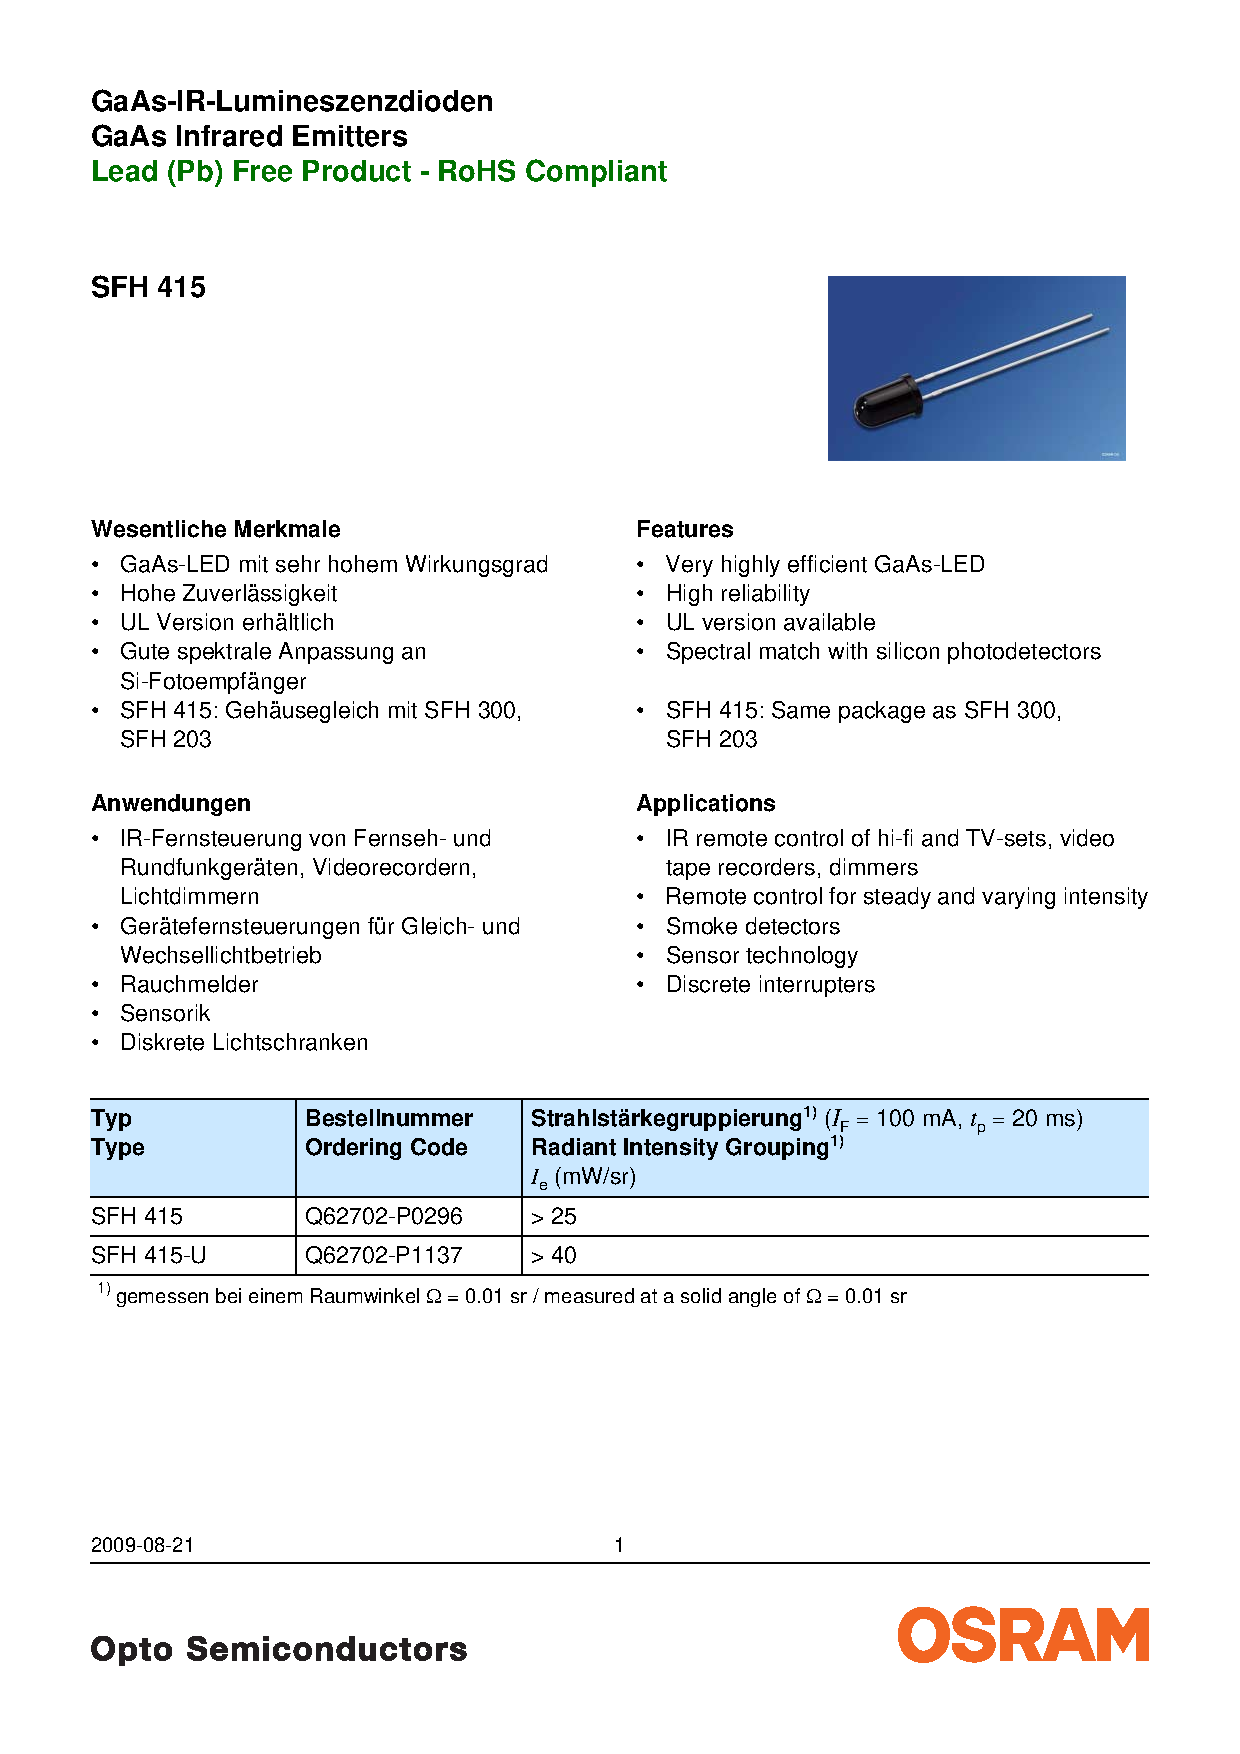
\includepdf[pages={1-3,5}]{docs/doc_IR_SFH415.pdf}

\end {document}